\documentclass{beamer}
\usepackage{listings}
\usepackage[utf8]{inputenc}
\usepackage[T1]{fontenc}
\usepackage{xcolor}

\definecolor{codegreen}{rgb}{0,0.6,0}
\definecolor{codegray}{rgb}{0.5,0.5,0.5}
\definecolor{codepurple}{rgb}{0.58,0,0.82}
\definecolor{backcolour}{rgb}{0.95,0.95,0.92}
\lstdefinestyle{mystyle}{
    backgroundcolor=\color{backcolour},
    commentstyle=\color{codegreen},
    keywordstyle=\color{magenta},
    numberstyle=\tiny\color{codegray},
    stringstyle=\color{codepurple},
    basicstyle=\ttfamily\footnotesize,
    breakatwhitespace=false,
    breaklines=true,
    captionpos=b,
    keepspaces=true,
    numbers=left,
    numbersep=5pt,
    showspaces=false,
    showstringspaces=false,
    showtabs=false,
    tabsize=2
}
\lstset{style=mystyle}


\title{An introduction to\\Neural Networks (NNs)}
\date{\today}
\author{Jorge Martín Pérez\\jmartinp@it.uc3m.es}

\usetheme{uc3m}

\begin{document}

\begin{frame}
\titlepage
\end{frame}

\setcounter{framenumber}{0}


\begin{frame}
    \frametitle{A neural network (NN)}
%\framesubtitle{The proof uses \textit{reductio ad absurdum}.}
    When we all think of NNs we have in mind this (maybe with a higher resolution image):
    \begin{figure}
        \centering
        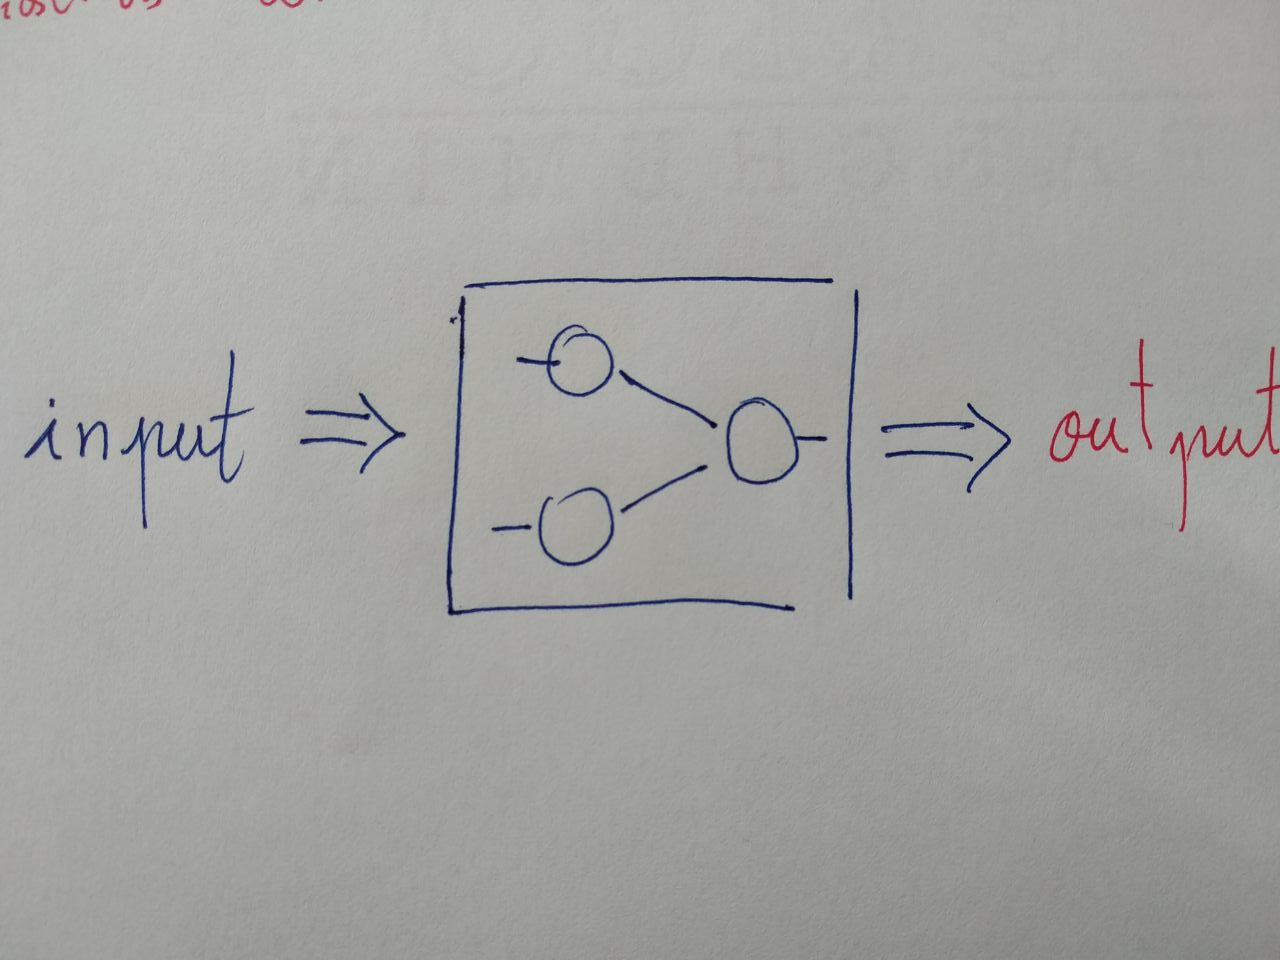
\includegraphics[width=0.6\textwidth]{img/black-box.jpg}
        \caption{}
        \label{fig:black-box}
    \end{figure}
\end{frame}

\begin{frame}
    \frametitle{They are trained!}
    What people imagine when ``data-scientists'' say they train a NN:
    \begin{figure}
        \centering
        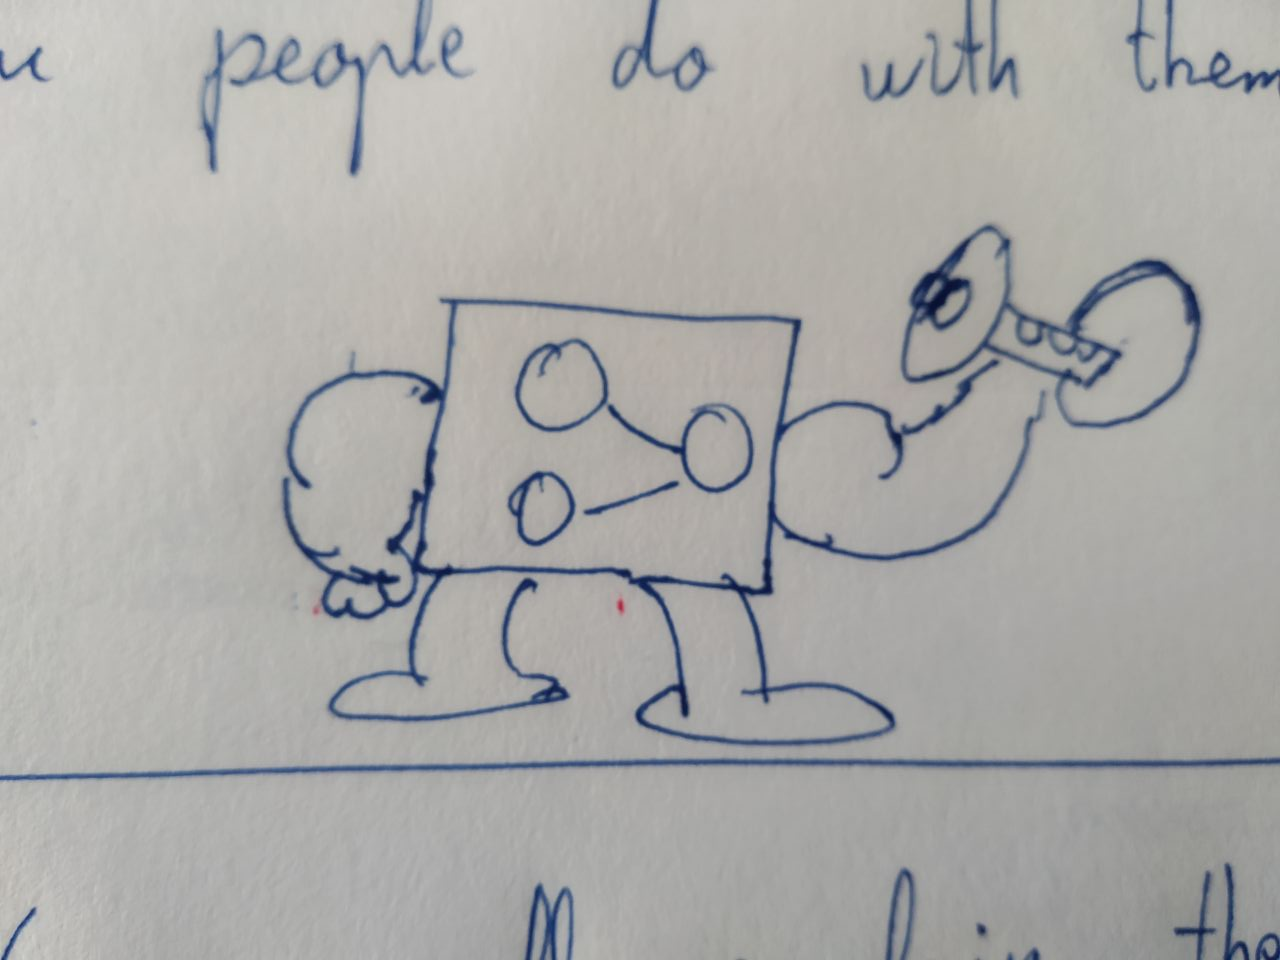
\includegraphics[width=0.6\textwidth]{img/trained-nn.jpg}
        \caption{trained-NN.jpg}
        \label{fig:trained-nn}
    \end{figure}
\end{frame}


\begin{frame}
    \frametitle{These slides}
    In these slides we'll try to bring some light to Figures~\ref{fig:black-box},\ref{fig:trained-nn}; i.e.:
    \begin{itemize}
        \item explain \textbf{how a NN works}; and
        \item how to \textbf{train} a NN.
    \end{itemize}
\end{frame}


\section{Motivation}
\begin{frame}
    \frametitle{\insertsection}
    \framesubtitle{guessing the ``function'' }

    So lets start talking about input $x$, and output $y$. Since highschool we learn to write it as:
    \begin{equation*}
        y = f(x)
    \end{equation*}

    \begin{figure}
        \centering
        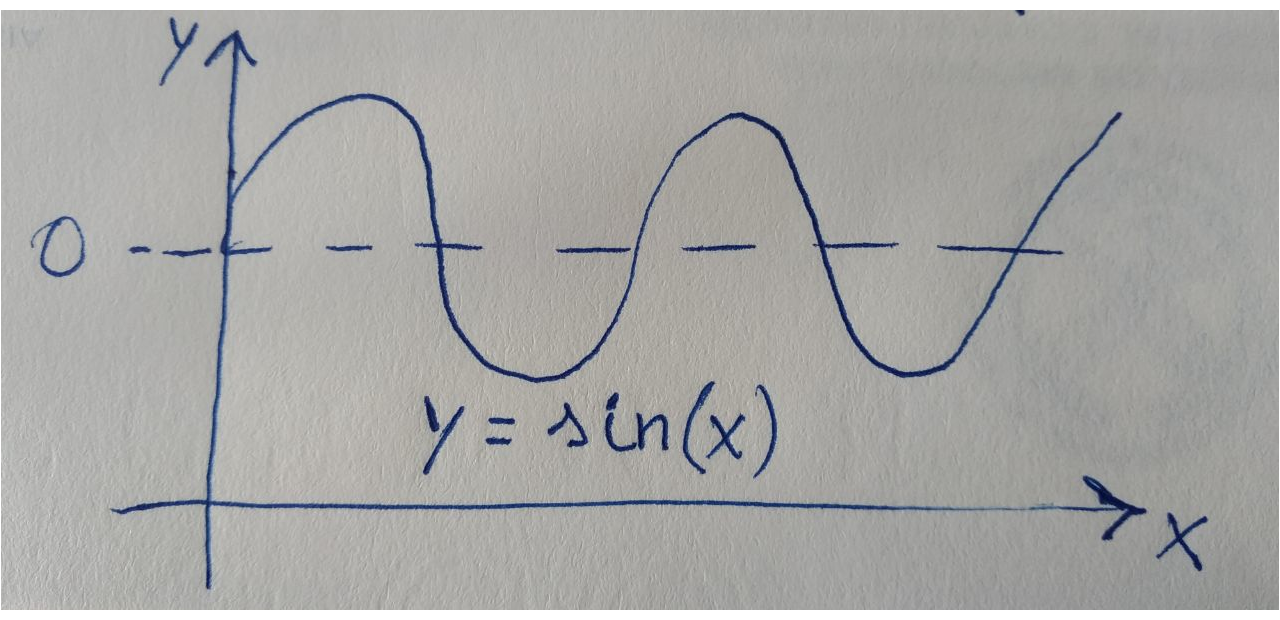
\includegraphics[width=0.6\textwidth]{img/sine.png}
        \caption{}
        \label{fig:sine}
    \end{figure}
\end{frame}


\begin{frame}
    \frametitle{\insertsection}
    \framesubtitle{guessing the ``function'' }

    Traditionally there has been different approaches
    to try to guess $f(x)$ given the input $x$:
    \begin{itemize}
        \item splines (numerical calculus);
        \item regression (statistics); and
        \item many others\footnote{the nicest way to say that no more come to my mind}.
    \end{itemize}
\end{frame}



\begin{frame}
    \frametitle{\insertsection}
    \framesubtitle{guessing the ``function'' }

    But when data patterns present non-linearities, things become difficult.

    \begin{figure}
        \centering
        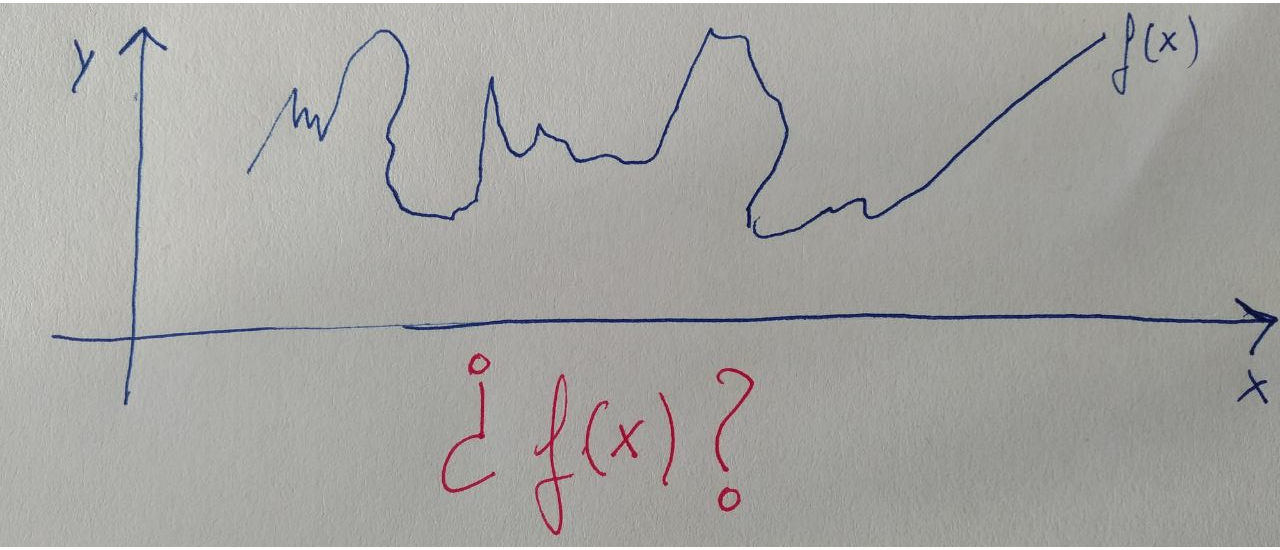
\includegraphics[width=0.8\textwidth]{img/strange-function.png}
        \caption{Try to guess this $f(x)$!}
        \label{fig:strange}
    \end{figure}
\end{frame}



\begin{frame}
    \frametitle{\insertsection}
    \framesubtitle{guessing the ``function'' }

    So is in situations like Figure~\ref{fig:strange} where NNs are quite useful.

    \begin{figure}
        \centering
        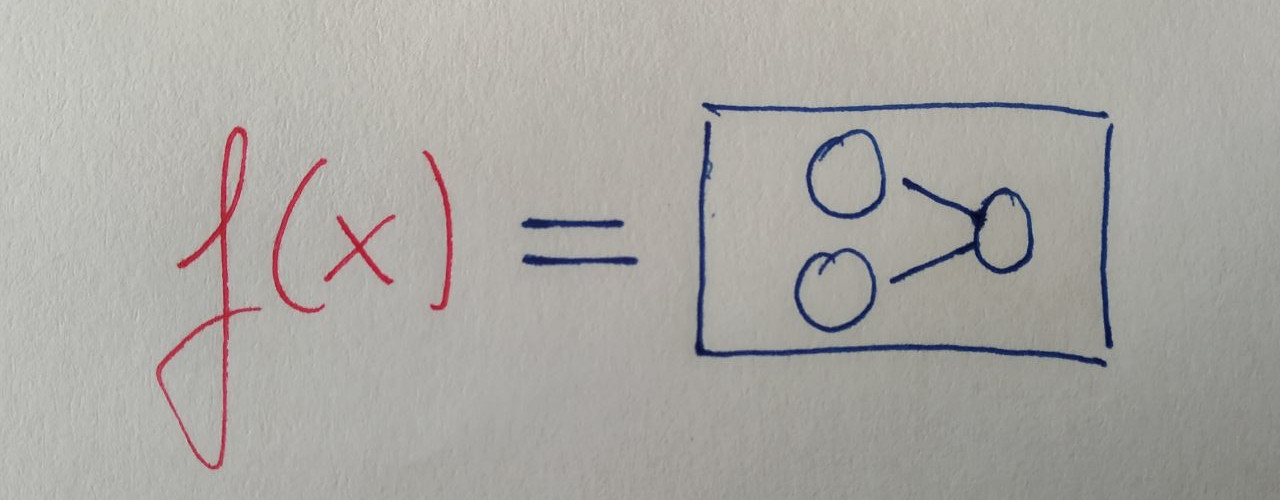
\includegraphics[width=0.8\textwidth]{img/fx-nn.jpg}
        \caption{The right box is a NN.}
        \label{fig:fx-nn}
    \end{figure}
\end{frame}


\section{Explaining a NN}
\subsection{A neuron}
\begin{frame}
    \frametitle{\insertsection}
    \framesubtitle{\insertsubsection}

    The balls inside the box of Figure~\ref{fig:fx-nn} are neurons, and probably you already knew that.

    \begin{figure}
        \centering
        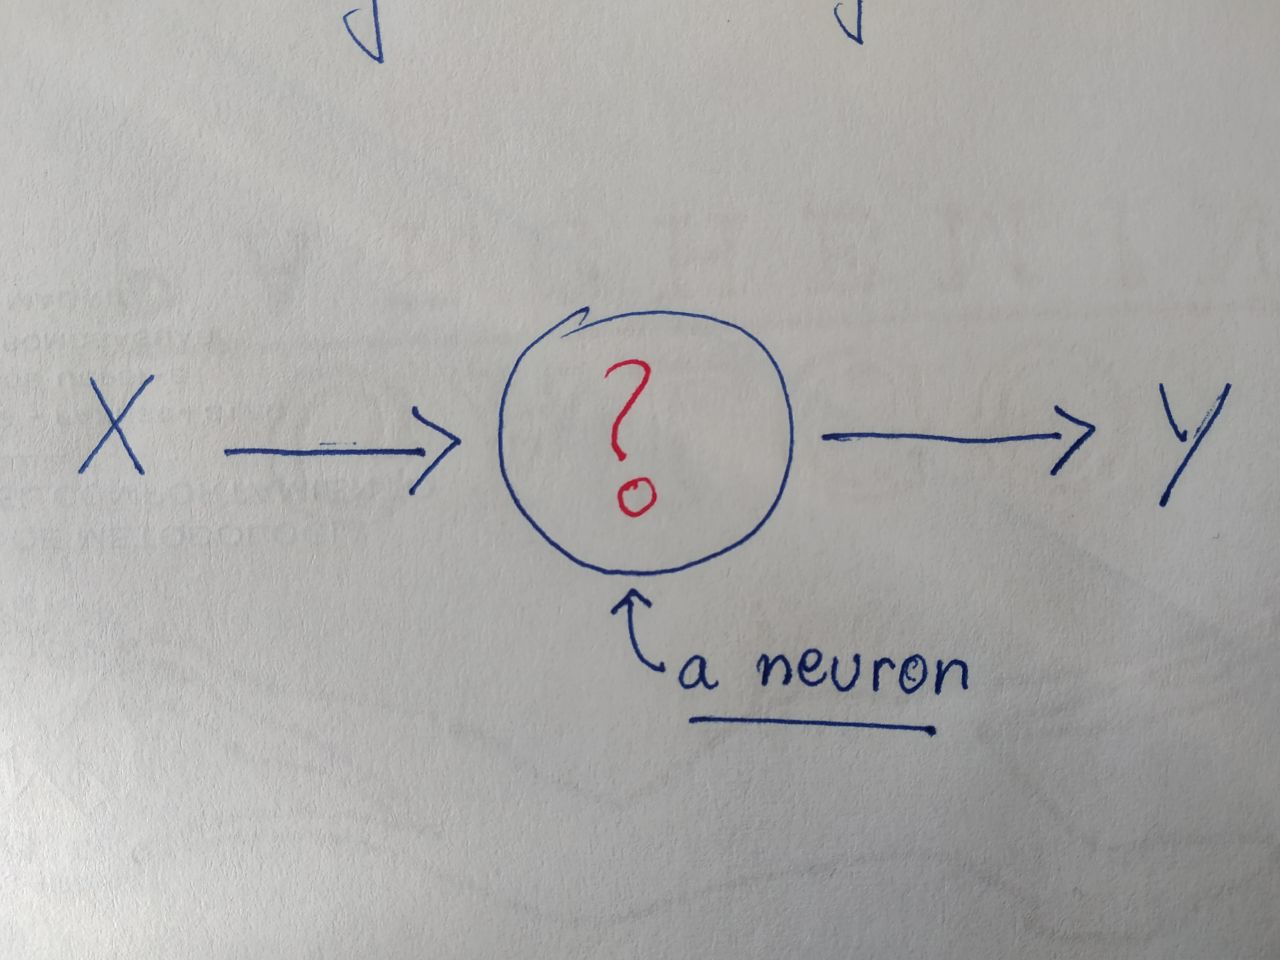
\includegraphics[width=0.6\textwidth]{img/neuron.jpg}
        \caption{Basically, a neuron takes a number $x$, and outputs another number $y$.}
        \label{fig:neuron}
    \end{figure}
\end{frame}

\begin{frame}
    \frametitle{\insertsection}
    \framesubtitle{\insertsubsection}

    A neuron will produce output $y$ using a function. A commonly used neuron, is the Rectifier Linear Unit (ReLU\footnote{It has nice properties for learning \href{http://tex.stackexchange.com/q/20800/5701}{\beamergotobutton{Wikipedia}}}):
    \begin{equation*}
        y=f(x)=\begin{cases}
            x,& x>0\\
            0, & x\le 0
        \end{cases}
    \end{equation*}
    \begin{figure}
        \centering
        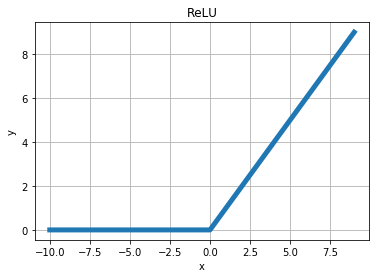
\includegraphics[width=0.35\textwidth]{img/relu.png}
        \caption{$ReLU(x)$}
        \label{fig:fx-nn}
    \end{figure}
\end{frame}




\begin{frame}
    \frametitle{\insertsection}
    \framesubtitle{}

    Ok, but a silly ReLU can't recognize my face, as some NNs do
    \begin{figure}
        \centering
        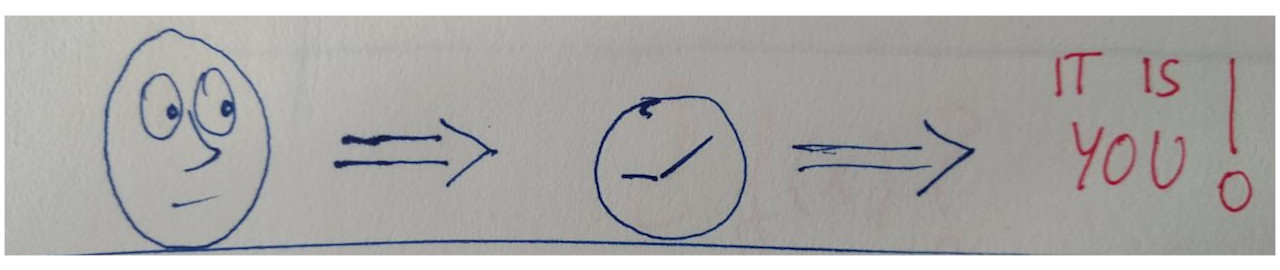
\includegraphics[width=\textwidth]{img/face.jpg}
        \caption{}
        \label{fig:face}
    \end{figure}
\end{frame}



\subsection{The weights}
\begin{frame}
    \frametitle{\insertsection}
    \framesubtitle{\insertsubsection}

    Right, one neuron cannot. But many of them can, and this is when \textbf{weights} come to the game!
    \begin{figure}
        \centering
        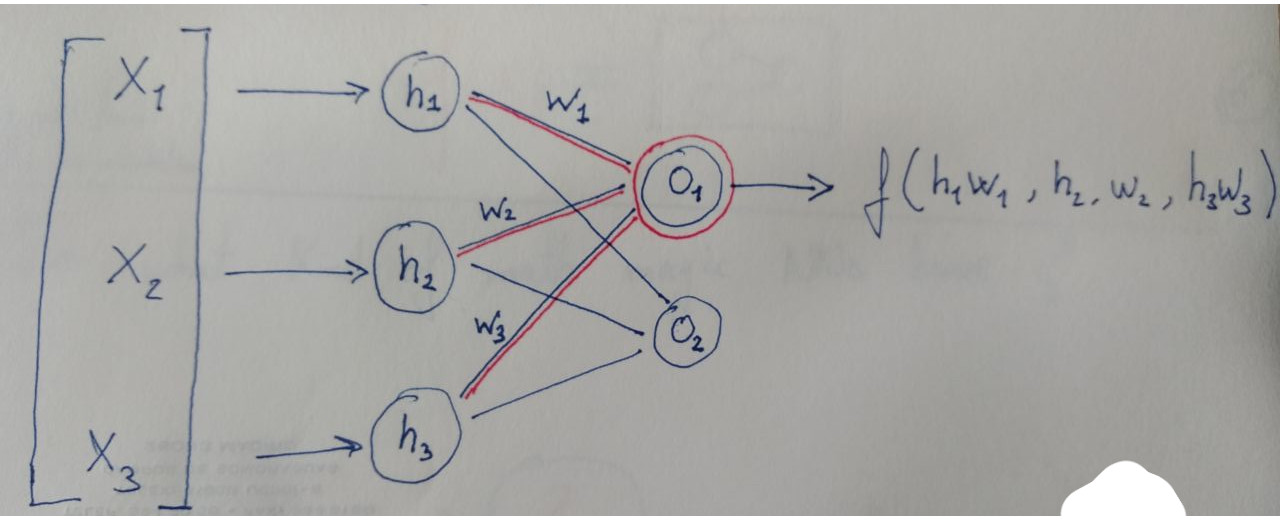
\includegraphics[width=\textwidth]{img/weights.jpg}
        \caption{$x$ input vector, $h_i$ hidden neurons, $o_i$ output neurons; and $f(\cdot)=o_i(\cdot)$}
        \label{fig:weights}
    \end{figure}
\end{frame}


\begin{frame}
    \frametitle{\insertsection}
    \framesubtitle{\insertsubsection}

    An example of a function for a given neuron output would be:
    \begin{equation*}
        f(h_1w_1,h_2w_2,h_3w_3) = ReLU(h_1w_1+h_2w_2+h_3w_3)
    \end{equation*}
\end{frame}



\begin{frame}
    \frametitle{\insertsection}
    \framesubtitle{\insertsubsection}

    Nice, so basically a NN takes an input vector and yields out an output vector!
    \begin{figure}
        \centering
        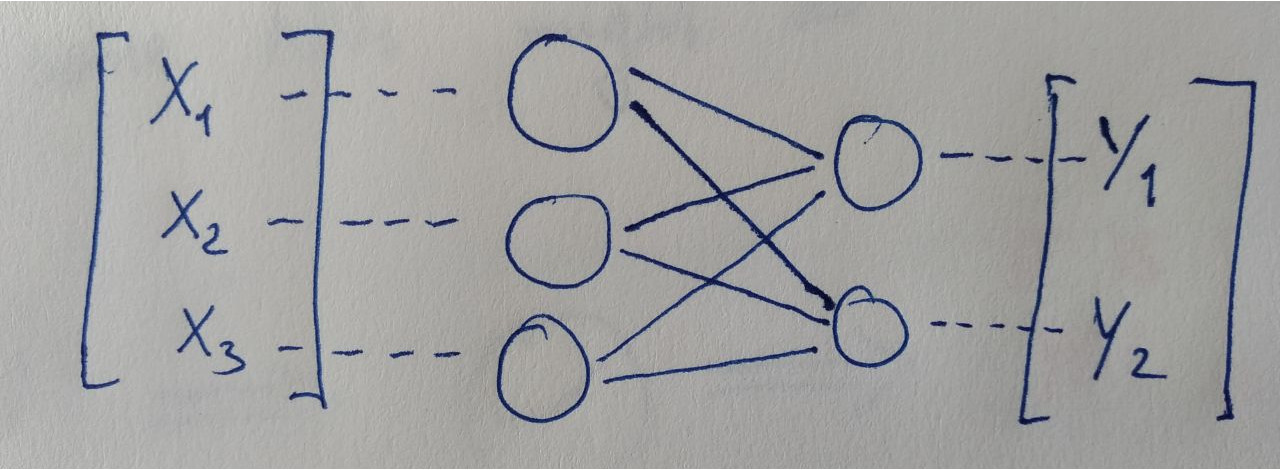
\includegraphics[width=0.7\textwidth]{img/vector-to-vector.jpg}
        \caption{}
        \label{fig:vector-to-vector}
    \end{figure}

    Yes, plus the NN does quite a \textbf{good at capturing non-linearities} (remember Figure~\ref{fig:strange})?
\end{frame}



\begin{frame}
    \frametitle{\insertsection}
    \framesubtitle{\insertsubsection}

    And how can a NN learn?
    \onslide<2->\begin{figure}
        \centering
        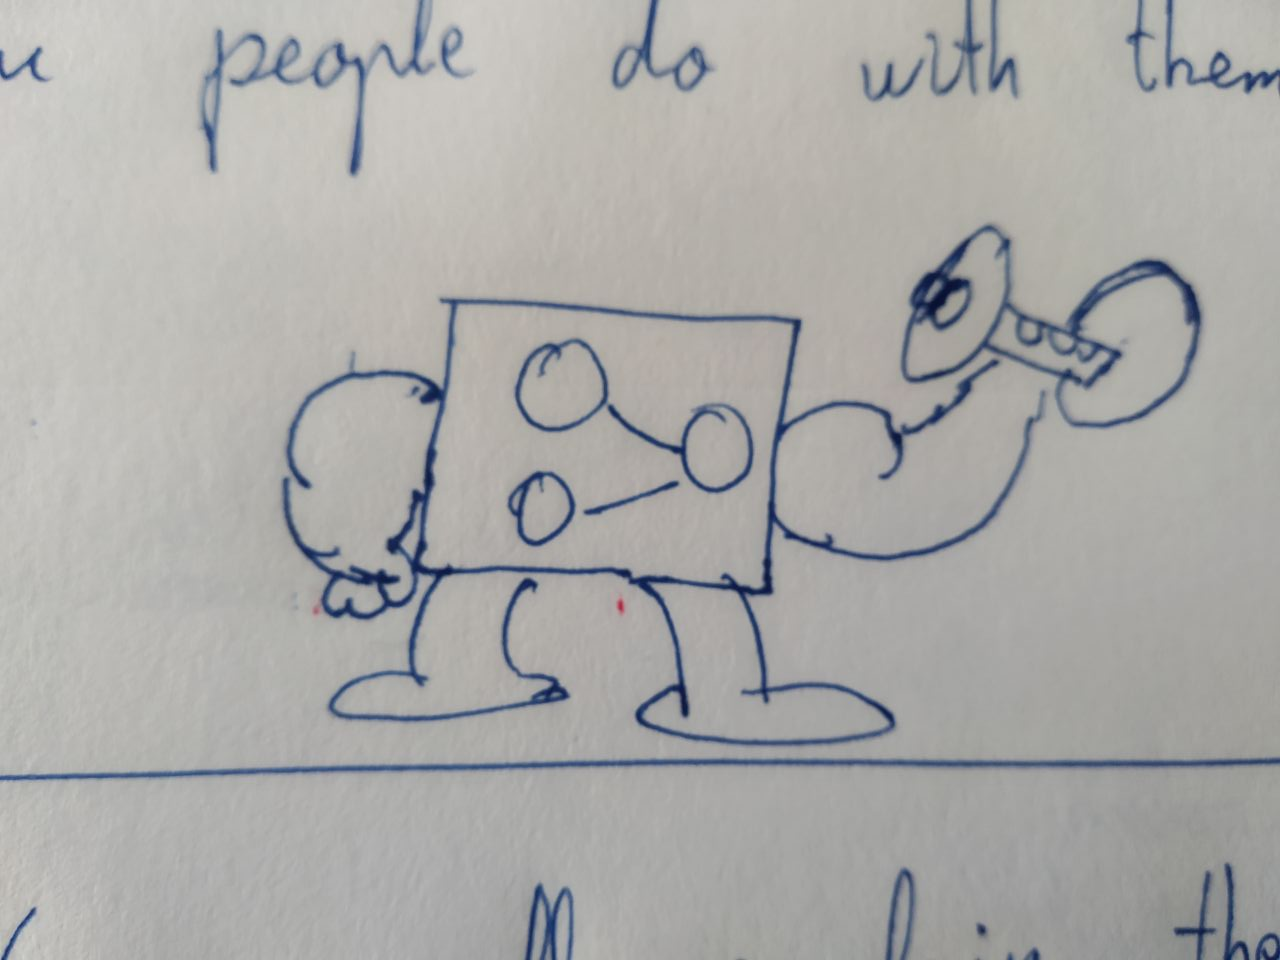
\includegraphics[width=0.7\textwidth]{img/trained-nn.jpg}
        \caption{The NN learns its weights with training!}
        \label{fig:trained-nn-2}
    \end{figure}
\end{frame}



\begin{frame}
    \frametitle{\insertsection}
    \framesubtitle{\insertsubsection}

    Lets start with an example.

    Imagine the zero-defect-manufacturing (ZDM) of 5G-DIVE.

    A camera checks a piece, and reports:
    \begin{itemize}
        \item $x_1\in[0,11]$ - horizontal-offset;
        \item $x_2\in[0,11]$ - vertical-offset; and
        \item $x_3\in[0,255]$ - black intensity (0-255).
    \end{itemize}
    and must decide
    \begin{itemize}
        \item $y_1\in\{0,1\}$ - piece needs corrections; and
        \item $y_2\in\{0,1\}$ - throw it to the trash.
    \end{itemize}
\end{frame}



\begin{frame}
    \frametitle{\insertsection}
    \framesubtitle{\insertsubsection}

    To train the network we need and historic of observations and the performed actions:
    \begin{equation*}
        (x_1=1,x_2=2,x_3=220)\qquad (\hat{y}_1=0,\hat{y}_2=1)
    \end{equation*}
    we denote with $\hat{y}$ what is commonly known as \textbf{labels}.
\end{frame}



\begin{frame}
    \frametitle{\insertsection}
    \framesubtitle{\insertsubsection}

    Imagine we have 200 observations, and not only the real values $(\hat{y}_1,\hat{y}_2)$, but the corresponding predictions $(y_1,y_2)$.

    \vfill
    During the training, we'd like to minimize:
    \begin{equation}
        MSE\left(\{y^i\}_i^{200},\{\hat{y}^i\}_i^{200}\right)=\frac{1}{200}\sum_i^{200} ||(\hat{y}_1^i,\hat{y}_2^i) - (y_1^i, y_2^i)||_2^2
        \label{eq:mse}
    \end{equation}
    this is nothing but the Mean Square Error (MSE)

\end{frame}




\begin{frame}
    \frametitle{\insertsection}
    \framesubtitle{\insertsubsection}

    Ok, but what does this have to do with the trainning and the weights?

    \onslide<2->{If we check Figure~\ref{fig:weights}, we can see that $o_1=y_1$ is written as:
    \begin{equation*}
        y_1 = o_1= f(h_1w_1, h_2w_2, h_3w_3)
    \end{equation*}
    }

    \onslide<3->{This means that the selection of $w_i$ affect how big is the prediction error (\ref{eq:mse})}

\end{frame}



\begin{frame}
    \frametitle{\insertsection}
    \framesubtitle{\insertsubsection}

    One can draw the prediction error (MSE in our case) as below.


    \begin{figure}
        \centering
        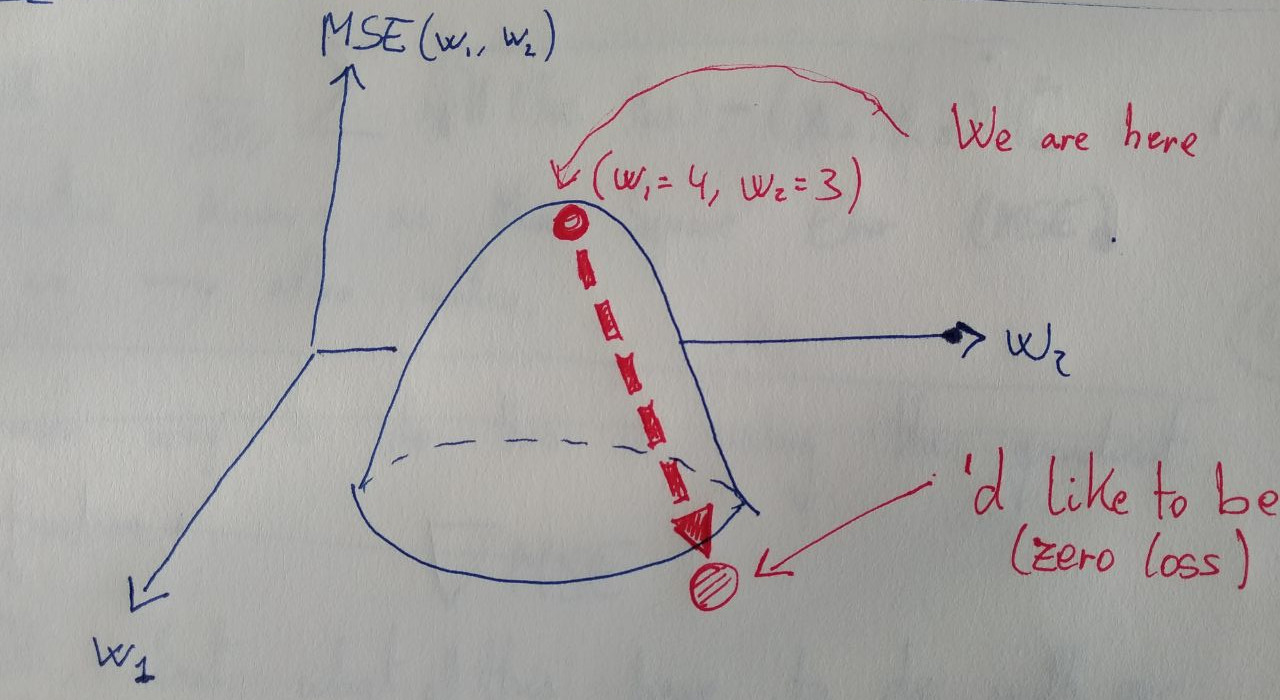
\includegraphics[width=0.9\textwidth]{img/gradient-descend.jpg}
        \caption{MSE as function of $w_1,w_2$}
        \label{fig:trained-nn-2}
    \end{figure}
\end{frame}



\begin{frame}
    \frametitle{\insertsection}
    \framesubtitle{\insertsubsection}

    Most of you have guessed it right, this is \textbf{gradient descend}, it is ML core idea, and we ``move'' the weights in the direction that minimizes the MSE:

    \begin{equation}
        (w_1',w_2',w_3') = (w_1,w_2,w_3) - \nabla_w MSE(\{y^i\}_i^{200},\{\hat{y}^i\}_i^{200})
    \end{equation}

    \vfill
    A quite known technique is Stochastic Gradient Descend (\textbf{SGD}), and existing methods are inspired in that one.
\end{frame}



\begin{frame}
    \frametitle{\insertsection}
    \framesubtitle{\insertsubsection}

    Back to the game: \underline{how do I use this}?
    \vfill

    Well, in your set of observations you have \textbf{batches}: lists of features with its respective labels:

    \begin{equation*}
        batch=\begin{cases}
            \text{features:} & \left[ {\color{blue}(x_1,x_2,x_3)}, {\color{red}(x_1,x_2,x_3)},\ldots \right],\\
            \text{labels:} & \left[ {\color{blue}(y_1,y_2)}, {\color{red}(y_1,y_2)},\ldots \right]
        \end{cases}
    \end{equation*}
\end{frame}


\begin{frame}
    \frametitle{\insertsection}
    \framesubtitle{\insertsubsection}

    You do a gradient-descend step ``a batch at a time''.

    Lets say we have our batch with 2 observations:
    \begin{equation*}
        batch=\begin{cases}
            \left[ {\color{blue}(x_1=1,x_2=3,x_3=220)}, {\color{red}(x_1=3,x_2=1,x_3=20)},\ldots \right]\\
            \left[ {\color{blue}(y_1=0,y_2=0)}, {\color{red}(y_1,y_2)},\ldots \right]
        \end{cases}
    \end{equation*}

    We plug these values in our network in next slide.
\end{frame}






\begin{frame}
    \frametitle{\insertsection}
    \framesubtitle{\insertsubsection}

    \begin{equation*}
        \begin{cases}
            \color{blue}y_1 =& \color{blue}ReLU(x_1=1)w_1+ReLU(x_2=2)w_2+ReLU(x_3=220)w_3 =\\
                             &\color{blue}= w_1 + 3w_2 + 220w_3\\
            \color{blue}y_2=& \ldots\\
            \color{red}y_1 =&\color{red} \ldots = 3w_1 + w_2 + 20w_3\\
            \color{red}y_2=& \ldots
        \end{cases}
    \end{equation*}

    \begin{figure}
        \centering
        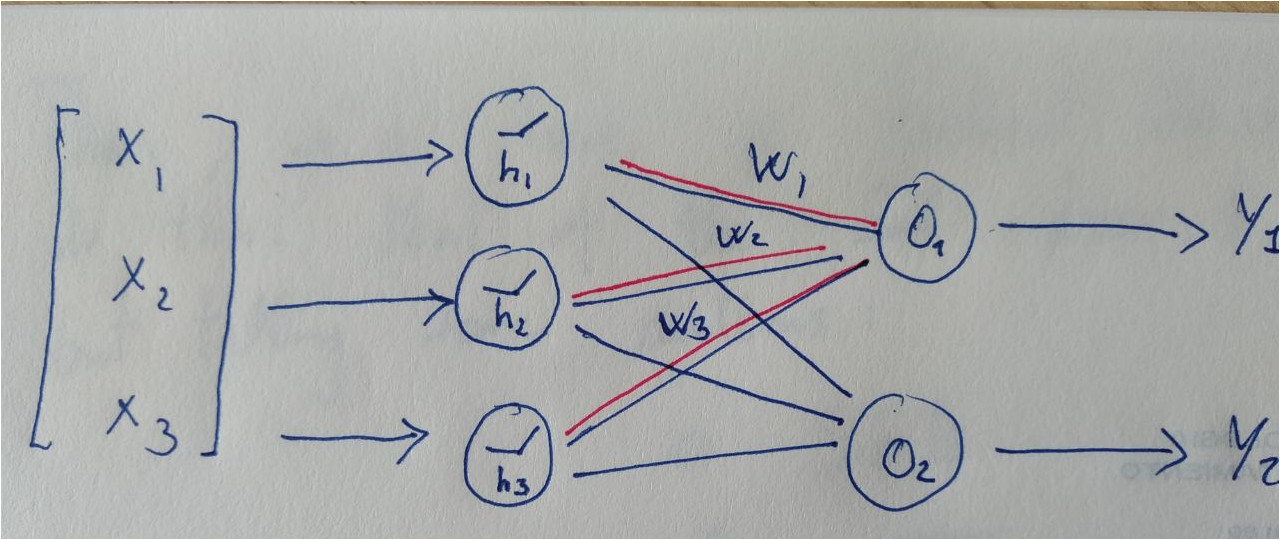
\includegraphics[width=0.7\textwidth]{img/nn-relu.jpg}
        \caption{}
        \label{fig:nn-relu}
    \end{figure}
\end{frame}





\begin{frame}
    \frametitle{\insertsection}
    \framesubtitle{\insertsubsection}

    If we plug above expressions in the MSE expression (\ref{eq:mse}), we have:
    \begin{align*}
        MSE({\color{blue} \hat{y},y},{\color{red} \hat{y},y})=& \frac{1}{2}\left( {\color{blue} || (\hat{y}_1, \hat{y}_2) - (y_1,y_2) ||_2^2} + {\color{red}|| (\hat{y}_1, \hat{y}_2) - (y_1,y_2) ||_2^2 } \right)=\\
                                                  &= \frac{1}{2} \big( {\color{blue}|| (0,1)-(w_1+3w_2+220w_3, \ldots) ||_2^2}\\
                                                  & \qquad + {\color{red}|| (0,0) - (3w_1+w_2+20w_3,\ldots) ||_2^2}\big) =\\
                                                  & \ldots \\
                                                  &- \onslide<2->{\text{\huge A MESS!}}
    \end{align*}
\end{frame}





\begin{frame}
    \frametitle{\insertsection}
    \framesubtitle{\insertsubsection}

    Happily, NNs atomatically do the job using \textbf{back-propagation}\footnote{\href{https://en.wikipedia.org/wiki/Backpropagation}{\beamergotobutton{Wikipedia}}}.
    \vfill

    \onslide<2->{In any case, imagine previous slide gave us:
        \begin{equation*}
            MSE({\color{blue} \hat{y},y},{\color{red} \hat{y},y})= w_2 + 4w_3
        \end{equation*}
        then, our batch would give as a gradient of
        \begin{equation*}
            \nabla_w MSE({\color{blue} \hat{y},y},{\color{red} \hat{y},y})= (0,1,4)
        \end{equation*}
        and we would update our weights (init as zero):
        \begin{equation*}
            (w_1',w_2',w_3') = (w_1=0,w_2=0,w_3=0)-\alpha (0,1,4)
        \end{equation*}
    }
\end{frame}




\begin{frame}
    \frametitle{\insertsection}
    \framesubtitle{\insertsubsection}
    Wait, what was that $\alpha$?

    \vspace{1em}
    \onslide<2->{
        it is the \textbf{learning rate}, i.e., how fast you want the NN to learn upon each batch update.

        Usually you decrease $\alpha$ as you advance in the training
    }
\end{frame}



\section{Conclusions}
\begin{frame}
    \frametitle{\insertsection}
    So lets recap what we've learned:
    \begin{enumerate}
        \item<1-> Our NN has weights $w_i$;
        \item<2-> Each training step uses a batch:
            \begin{itemize}
                \item inputs: $[{\color{blue}(x_1,x_2,x_3)}, {\color{red}(x_1,x_2,x_3)}]$
                \item labels: $[{\color{blue}(y_1,y_2)}, {\color{red}(y_1,y_2)}]$
            \end{itemize}
        \item<3-> For each \textbf{batch} we see how good is the prediction:
            \begin{equation*}
                MSE({\color{blue} \hat{y},y},{\color{red} \hat{y},y})= \frac{1}{2}\left( {\color{blue} || (\hat{y}_1, \hat{y}_2) - (y_1,y_2) ||_2^2} + {\color{red}|| (\hat{y}_1, \hat{y}_2) - (y_1,y_2) ||_2^2 } \right)
            \end{equation*}
        \item<4-> We update $w_i$ using gradient descend based on MSE:
            \begin{equation*}
                (w_1',w_2',w_3') = (w_1,w_2,w_3) - \alpha \nabla_w MSE({\color{blue} \hat{y},y},{\color{red} \hat{y},y})
            \end{equation*}
    \end{enumerate}
\end{frame}


\section{Tensorflow implementation}
\begin{frame}[fragile]
    \frametitle{\insertsection}
    \vfill

    \textit{Talk is cheap, show me the code}

    \hfill Linus Torvalds

    {\onslide<2->\hfill Luca Cominardi
    }
    \vfill
\end{frame}


\begin{frame}[fragile]
    \frametitle{\insertsection}
    \begin{figure}
        \centering
        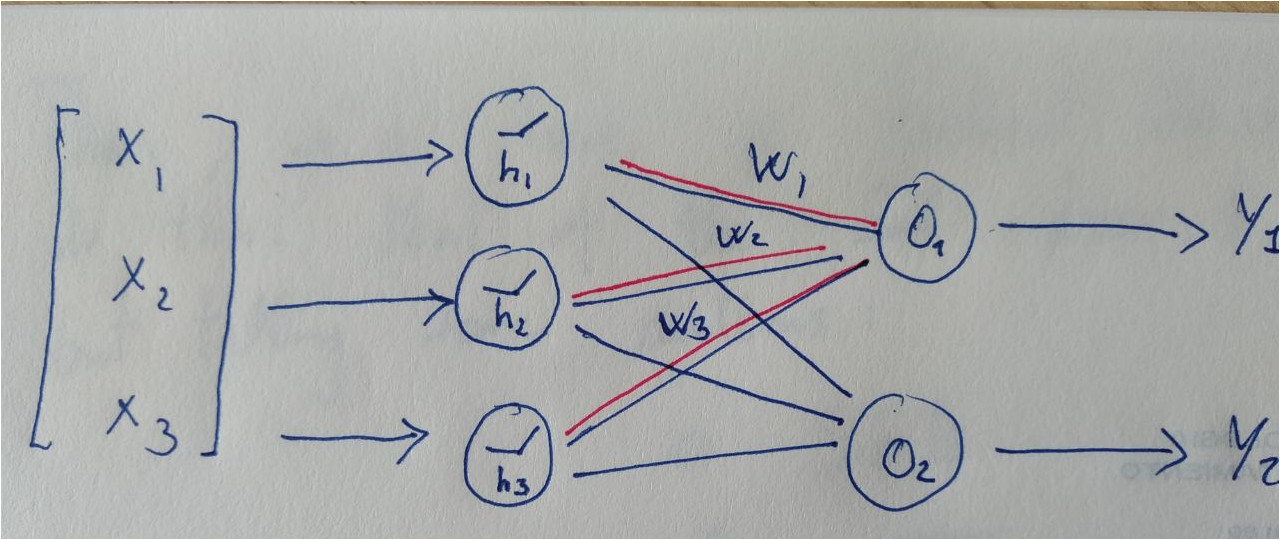
\includegraphics[width=0.7\textwidth]{img/nn-relu.jpg}
        \caption{}
        \label{fig:nn-relu2}
    \end{figure}

        \begin{lstlisting}[language=Python]
NN_model = tf.keras.Sequential([
  # (h1,h2,h3)
  tf.keras.layers.Activation('relu', input_shape=[3]),
  # (y1, y2)
  tf.keras.layers.Dense(2, use_bias=False),  
])\end{lstlisting}

\end{frame}


\begin{frame}
    \frametitle{\insertsection}
    You can find a complete implementation of the ZDM example in \href{https://github.com/MartinPJorge/nn-intro-slides/blob/master/zdm.ipynb}{\beamergotobutton{GitHub}}
    \vfill
    \begin{figure}
        \centering
        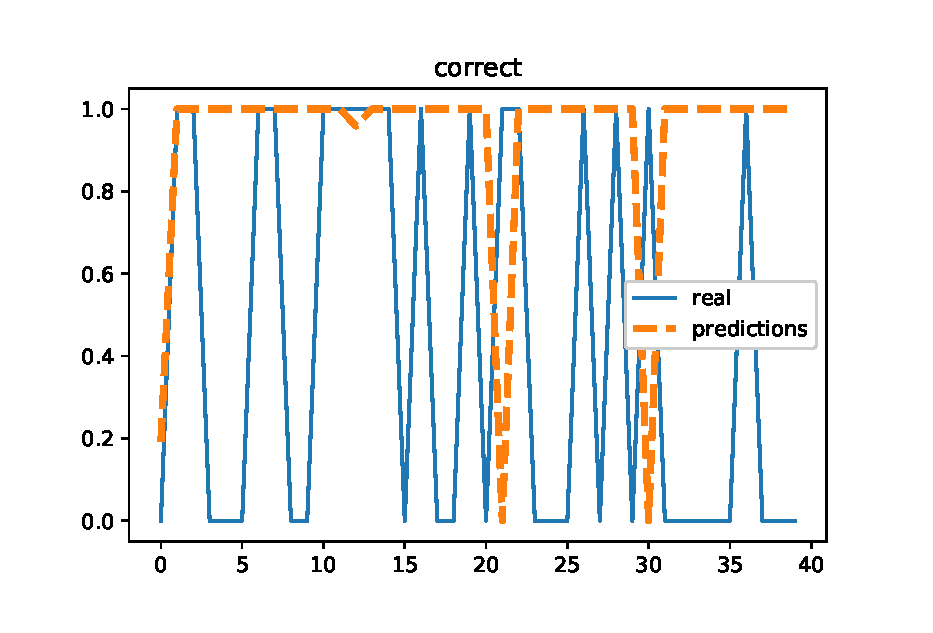
\includegraphics[width=0.8\textwidth]{img/correct.eps}
        \caption{Predicted $y_1$ output in ZDM}
        \label{fig:nn-relu2}
    \end{figure}
\end{frame}



\end{document}
